\documentclass[11pt,a4paper]{article}
\usepackage{gtu-el-yazisi}
\begin{document}
\notbilgi{Analog Haberleşme}{İşaretler, güç/enerji, temel işaretler ve sistemler}{Ders2.pdf}

\sayfa{1}
\section{Ders 2}
\textbf{Enerji:}
\[ E_x = \lim_{T\to\infty}\int_{-T/2}^{T/2}|x(t)|^2\,dt = \int_{-\infty}^{\infty}|x(t)|^2\,dt \]
$E_x<\infty \Rightarrow$ Enerji işaretidir

\textbf{Güç:}
\[ P_x = \lim_{T\to\infty}\frac{1}{T}\int_{-T/2}^{T/2}|x(t)|^2\,dt \]
$0<P_x<\infty \Rightarrow$ Güç işaretidir

\[ x(t)=\begin{cases} A\cos(2\pi f_0 t+\theta)\\ A\sin(2\pi f_0 t+\theta)\end{cases} \longrightarrow\quad P_x=\frac{A^2}{2} \]
$T_0=\dfrac{1}{f_0}$ periyottur.

Periyodik $\Rightarrow P_x=\dfrac{1}{T_0}\displaystyle\int_{T_0}|x(t)|^2\,dt$

\textcolor{kirmizikalem}{\textbf{ispat}}
\begin{align*}
P_x &= \frac{1}{T_0}\int_{T_0}A^2\cos^2(2\pi f_0 t+\theta)\,dt = \frac{A^2}{2T_0}\int_{-T_0/2}^{T_0/2}\left[1+\cos(4\pi f_0 t+2\theta)\right]dt \\
&= \frac{A^2}{2T_0}\left[T_0+\underbrace{\int_{-T_0/2}^{T_0/2}\cos(4\pi f_0 t+2\theta)\,dt}_{0}\right]
\end{align*}
$\ast$ sinüsoidal işaretlerin bir periyot boyunca integrali 0'dır.

\elcizimi[0.4]{sekiller/Ders2-s1-1.png}[1]
\formulkutu{P_x=\frac{A^2}{2}}

\begin{ornek}
  Lathi'den örnek \\
  $x(t)=c_1\cos(2\pi f_1 t+\theta_1)+c_2\cos(2\pi f_2 t+\theta_2)\,,\quad f_1\neq f_2$ \\
  $P_x=\,?$ \\
  Bir işaretin periyodunu bileşenlerinin periyodlarının en küçük ortak katlarıyla bulunabilir
\end{ornek}

\sayfa{2}
\[ P_x = \lim_{T\to\infty}\frac{1}{T}\int_{-T/2}^{T/2}|x(t)|^2\,dt \]
\begin{align*}
&= \underbrace{\lim_{T\to\infty}\frac{1}{T}\int_{-T/2}^{T/2}c_1^2\cos^2(2\pi f_1 t+\theta_1)\,dt}_{c_1^2/2} \\
&\quad + \underbrace{\lim_{T\to\infty}\frac{1}{T}\int_{-T/2}^{T/2}c_2^2\cos^2(2\pi f_2 t+\theta_2)\,dt}_{c_2^2/2} \\
&\quad + \lim_{T\to\infty}\frac{1}{T}\,2c_1c_2\int_{-T/2}^{T/2}\cos(2\pi f_1 t+\theta_1)\cos(2\pi f_2 t+\theta_2)\,dt
\end{align*}
\begin{align*}
&\lim_{T\to\infty}\frac{1}{T}\,c_1c_2\int_{-T/2}^{T/2}\Big[\underbrace{\cos\big(2\pi(f_1+f_2)t+\theta_1+\theta_2\big)}_{0} \\
&\qquad +\underbrace{\cos\big(2\pi(f_1-f_2)t+\theta_1-\theta_2\big)}_{0}\Big]dt
\end{align*}
\formulkutu{\cos\alpha\cdot\cos\beta=\frac{1}{2}\Big[\cos(\alpha+\beta)+\cos(\alpha-\beta)\Big]}
\textcolor{kirmizikalem}{çünkü sinüsoidal} $\;\searrow\;$ \textcolor{murekkep}{burdan bu terim gelir}
\[ \Rightarrow\quad P_x=\begin{cases}
  \dfrac{c_1^2}{2}+\dfrac{c_2^2}{2}, & f_1\neq f_2 \\[3mm]
  \dfrac{c_1^2}{2}+\dfrac{c_2^2}{2}+c_1c_2\cos(\theta_1-\theta_2), & f_1=f_2
\end{cases} \]

\textbf{Sonuçlar}

$x(t)=x_1(t)+x_2(t) \Rightarrow P_x\neq P_{x_1}+P_{x_2}$

\hspace{3cm}compact fourier açılımı $\swarrow$
\[ x(t)=\sum_{n=1}^{\infty}c_n\cos(2\pi f_n t+\theta_n) \Rightarrow P_x=\frac{1}{2}\sum_{n=1}^{\infty}c_n^2 \qquad i\neq j,\ f_i\neq f_j \]
\hspace{6cm}(Parseval teoremi)

\begin{ornek}
  $x(t)=Ae^{j2\pi f_0 t}$
  \begin{align*}
    P_x &= \frac{1}{T_0}\int_{-T_0/2}^{T_0/2}|x(t)|^2\,dt = \frac{1}{T_0}\int_{-T_0/2}^{T_0/2}\underbrace{\left|Ae^{j2\pi f_0 t}\right|}_{A}{}^{2}dt \\
    &= \frac{1}{T_0}\int_{-T_0/2}^{T_0/2}|A|^2\,dt = |A|^2
  \end{align*}
  \formulkutu{\begin{aligned}
    z=x+jy&=|z|e^{j\theta}\\
    |z|&=\sqrt{x^2+y^2}\\
    \theta&=\arctan\frac{y}{x}\\
    |z_1\cdot z_2|&=|z_1||z_2|\\
    \bigl|Ae^{j2\pi f_0 t}\bigr|&=|A|\,\underbrace{\bigl|e^{j\overbrace{2\pi f_0 t}^{\alpha}}\bigr|}_{\cos(\alpha)+j\sin(\alpha)}
  \end{aligned}}
\end{ornek}

\sayfa{3}
\section{Bazı önemli işaretler}
\subsection{Sinüsoidal işaretler}
\[ x(t)=\underbrace{A}_{\substack{\text{Genlik}\\\text{(Amplitude)}}}\cos\Bigl(2\pi\,\overbrace{f_0}^{\text{frekans }(\mathrm{Hz}=\frac{1}{\mathrm{s}})}\,t+\underbrace{\theta}_{\substack{\text{Faz (rad)}\\\text{(phase)}}}\Bigr) \]
A güç veya enerji işaretin genliği ile orantılıdır

\subsection{Kompleks üstel işaretler}
\[ x(t)=A\,e^{j(2\pi f_0 t+\theta)} \]

\subsection{Birim Basamak İşareti}
(Unit step signal)

\noindent
\begin{minipage}[c]{0.42\linewidth}
  \[ u(t)=\begin{cases} 1 & t\ge 0 \\ 0 & t<0 \end{cases} \]
\end{minipage}\hfill
\begin{minipage}[c]{0.54\linewidth}
  \centering
  \begin{tikzpicture}
    \begin{axis}[width=6.6cm, height=3.6cm, xmin=-1.3, xmax=2.6, ymin=-0.3, ymax=1.45,
        xtick=\empty, ytick={1}, ylabel={$u(t)$}]
      \addplot[murekkep, line width=1.2pt] coordinates {(-1.3,0) (0,0) (0,1) (2.6,1)};
    \end{axis}
  \end{tikzpicture}
\end{minipage}

$a>0 \qquad u(at)=u(t)$

\begin{ornek}
  $x(t)=e^{-a|t|}\,u(t),\quad a>0$

  \medskip
  \noindent
  \begin{minipage}[c]{0.48\linewidth}
    \centering
    \begin{tikzpicture}
      \begin{axis}[width=6.2cm, height=3.4cm, xmin=-3.2, xmax=3.4, ymin=-0.1, ymax=1.35,
          xtick=\empty, ytick={1}, ylabel={$e^{-a|t|}$}]
        \addplot[murekkep, line width=1.2pt, domain=-3:3, samples=70] {exp(-abs(x))};
      \end{axis}
    \end{tikzpicture}
  \end{minipage}\hfill
  \begin{minipage}[c]{0.48\linewidth}
    \centering
    \begin{tikzpicture}
      \begin{axis}[width=6.2cm, height=3.4cm, xmin=-2.2, xmax=3.0, ymin=-0.2, ymax=1.35,
          xtick=\empty, ytick={1}, ylabel={$u(t)$}]
        \addplot[murekkep, line width=1.2pt] coordinates {(-2.2,0) (0,0) (0,1) (2.2,1)};
      \end{axis}
    \end{tikzpicture}
  \end{minipage}

  \medskip
  \noindent
  \begin{minipage}[c]{0.48\linewidth}
    \centering
    \begin{tikzpicture}
      \begin{axis}[width=6.2cm, height=3.4cm, xmin=-2.2, xmax=3.4, ymin=-0.15, ymax=1.35,
          xtick=\empty, ytick={1}, ylabel={$x(t)=e^{-a|t|}u(t)$}]
        \addplot[murekkep, line width=1.2pt] coordinates {(-2.2,0) (0,0) (0,1)};
        \addplot[murekkep, line width=1.2pt, domain=0:3.1, samples=50] {exp(-x)};
      \end{axis}
    \end{tikzpicture}
  \end{minipage}\hfill
  \begin{minipage}[c]{0.48\linewidth}
    \[ x(t)=\begin{cases} e^{-at}, & t\ge 0 \\ 0, & t<0 \end{cases} \]
  \end{minipage}
\end{ornek}

\sayfa{4}
\subsection{Dikdörtgen Darbe işareti}
(Rectangular pulse Signal)

\noindent
\begin{minipage}[c]{0.56\linewidth}
  \[ \mathrm{rect}(t)=\Pi(t)=\begin{cases} 1, & -\tfrac{1}{2}\le t\le\tfrac{1}{2} \\ 0, & \text{Diğer}\end{cases} \]
\end{minipage}\hfill
\begin{minipage}[c]{0.4\linewidth}
  \centering
  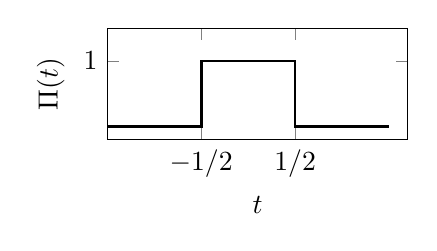
\begin{tikzpicture}
    \begin{axis}[width=5.4cm, height=3cm, xmin=-1.5, xmax=1.7, ymin=-0.2, ymax=1.5,
        xtick={-0.5,0.5}, xticklabels={$-1/2$,$1/2$}, ytick={1}, xlabel={$t$}, ylabel={$\Pi(t)$}]
      \addplot[black, line width=1pt] coordinates {(-1.5,0) (-0.5,0) (-0.5,1) (0.5,1) (0.5,0) (1.5,0)};
    \end{axis}
  \end{tikzpicture}
\end{minipage}

\[ \Pi(t)=u\!\left(t+\tfrac{1}{2}\right)-u\!\left(t-\tfrac{1}{2}\right) \]
\begin{center}
  \begin{tikzpicture}
    \begin{axis}[width=7.6cm, height=4.2cm, xmin=-2, xmax=2.2, ymin=-1.5, ymax=1.5,
        xtick=\empty, ytick=\empty]
      \addplot[kirmizikalem!55, line width=1.2pt] coordinates {(-2,0) (-0.5,0) (-0.5,1) (2,1)};
      \addplot[kirmizikalem, line width=1.2pt] coordinates {(-2,0) (0.5,0) (0.5,-1) (2,-1)};
      \node[kirmizikalem!55, font=\small] at (axis cs:1.2,1.35) {$u(t+\frac{1}{2})$};
      \node[kirmizikalem, font=\small] at (axis cs:1.4,-1.4) {$-u(t-\frac{1}{2})$};
    \end{axis}
  \end{tikzpicture}
\end{center}

\begin{ornek}
  $x(t)=2\,\Pi\Bigl(\underbrace{\tfrac{t-3}{6}}_{\frac{1}{6}(t-3)}\Bigr)-\Pi\Bigl(\underbrace{\tfrac{t-3}{4}}_{\frac{1}{4}(t-3)}\Bigr)$ \quad çiziniz

  \medskip
  \noindent
  \begin{minipage}[c]{0.48\linewidth}
    \centering
    \begin{tikzpicture}
      \begin{axis}[width=6.2cm, height=3.2cm, xmin=-4.5, xmax=4.8, ymin=-0.2, ymax=1.5,
          xtick={-3,3}, ytick=\empty, ylabel={$\Pi\bigl(\frac{1}{6}t\bigr)$}]
        \addplot[kirmizikalem!55, line width=1.2pt] coordinates {(-3,0) (-3,1) (3,1) (3,0)};
      \end{axis}
    \end{tikzpicture}
  \end{minipage}\hfill
  \begin{minipage}[c]{0.48\linewidth}
    \centering
    \begin{tikzpicture}
      \begin{axis}[width=6.2cm, height=3.2cm, xmin=-1.5, xmax=7.6, ymin=-0.3, ymax=2.7,
          xtick={6}, ytick={2}, ylabel={$2\Pi\bigl(\frac{t-3}{6}\bigr)$}]
        \addplot[kirmizikalem!55, line width=1.2pt] coordinates {(0,0) (0,2) (6,2) (6,0)};
      \end{axis}
    \end{tikzpicture}
  \end{minipage}

  \medskip
  \noindent
  \begin{minipage}[c]{0.48\linewidth}
    \centering
    \begin{tikzpicture}
      \begin{axis}[width=6.2cm, height=3.2cm, xmin=-3.5, xmax=3.8, ymin=-0.2, ymax=1.5,
          xtick={-2,2}, xticklabels={$-2$,$+2$}, ytick=\empty, ylabel={$\Pi\bigl(\frac{1}{4}t\bigr)$}]
        \addplot[kirmizikalem!55, line width=1.2pt] coordinates {(-2,0) (-2,1) (2,1) (2,0)};
      \end{axis}
    \end{tikzpicture}
  \end{minipage}\hfill
  \begin{minipage}[c]{0.48\linewidth}
    \centering
    \begin{tikzpicture}
      \begin{axis}[width=6.2cm, height=3.2cm, xmin=-1.5, xmax=6.8, ymin=-1.4, ymax=0.6,
          xtick=\empty, ytick={-1}, ylabel={$-\Pi\bigl(\frac{t-3}{4}\bigr)$}]
        \addplot[kirmizikalem!55, line width=1.2pt] coordinates {(1,0) (1,-1) (5,-1) (5,0)};
        \node[kirmizikalem!55, font=\small] at (axis cs:1,0.3) {$1$};
        \node[kirmizikalem!55, font=\small] at (axis cs:5,0.3) {$5$};
      \end{axis}
    \end{tikzpicture}
  \end{minipage}
\end{ornek}

\sayfa{5}
\begin{center}
  \begin{tikzpicture}
    \begin{axis}[width=7.4cm, height=3.6cm, xmin=-0.4, xmax=7.2, ymin=-0.8, ymax=2.7,
        xtick={1,5,6}, ytick={1,2}, xlabel={$t$}, ylabel={$x(t)$}]
      \addplot[kirmizikalem!55, line width=1.2pt] coordinates {(0,2) (1,2) (1,1) (5,1) (5,2) (6,2) (6,0)};
    \end{axis}
  \end{tikzpicture}
\end{center}

\noindent
\begin{minipage}[c]{0.5\linewidth}
  \[ \textcolor{kirmizikalem}{\ast}\ \ \Pi(t)=\begin{cases} 1 & -\tfrac{1}{2}\le t\le\tfrac{1}{2} \\ 0 & \text{diğer}\end{cases} \]
\end{minipage}\hfill
\begin{minipage}[c]{0.46\linewidth}
  \centering
  \begin{tikzpicture}
    \begin{axis}[width=5.8cm, height=3cm, xmin=-1.6, xmax=1.8, ymin=-0.3, ymax=1.5,
        xtick={-0.5,0.5}, xticklabels={$-1/2$,$1/2$}, ytick={1}]
      \addplot[kirmizikalem!55, line width=1.2pt] coordinates {(-0.5,0) (-0.5,1) (0.5,1) (0.5,0)};
    \end{axis}
  \end{tikzpicture}
\end{minipage}

\noindent
\begin{minipage}[c]{0.5\linewidth}
  \[ \Pi\!\left(\tfrac{t}{\tau}\right)=\begin{cases} 1, & -\tfrac{\tau}{2}\le t\le\tfrac{\tau}{2} \\ 0, & \text{diğer}\end{cases} \]
\end{minipage}\hfill
\begin{minipage}[c]{0.46\linewidth}
  \centering
  \begin{tikzpicture}
    \begin{axis}[width=5.8cm, height=3.4cm, xmin=-1.6, xmax=1.8, ymin=-0.9, ymax=1.5,
        xtick={-1,1}, xticklabels={$-\tau/2$,$\tau/2$}, ytick={1}]
      \addplot[kirmizikalem!55, line width=1.2pt] coordinates {(-1,0) (-1,1) (1,1) (1,0)};
      \draw[Stealth-Stealth, kirmizikalem!55, line width=0.8pt] (axis cs:-1,-0.62) -- (axis cs:1,-0.62)
        node[midway, below] {$\tau$};
    \end{axis}
  \end{tikzpicture}
\end{minipage}

\subsection{Üçgen darbe işareti}
(Triangular Pulse Signal)

\noindent
\begin{minipage}[c]{0.4\linewidth}
  \centering
  \begin{tikzpicture}
    \begin{axis}[width=5.8cm, height=3.2cm, xmin=-1.6, xmax=1.9, ymin=-0.3, ymax=1.4,
        xtick={-1,0,1}, ytick={1}]
      \addplot[kirmizikalem!55, line width=1.2pt] coordinates {(-1,0) (0,1) (1,0)};
    \end{axis}
  \end{tikzpicture}
\end{minipage}\hfill
\begin{minipage}[c]{0.56\linewidth}
  \[ \Lambda(t)=\begin{cases} t+1 & -1\le t\le 0 \\ -t+1 & 0\le t\le 1 \\ 0 & \text{Diğer}\end{cases} \]
\end{minipage}

\medskip
\noindent\textbf{Doğrunun denklemi}
\[ y=\overbrace{m}^{\text{eğim}}\,t+n \]
$t_1,y_1\rightarrow$ \qquad $t_2,y_2\rightarrow$

\[ \Lambda(t)=\begin{cases} 1-|t|, & \underbrace{|t|\le 1}_{-1\le t\le 1} \\ 0, & \text{diğer}\end{cases} \]

\[ \Lambda(t)=\Pi(t)\circledast\Pi(t) \qquad\longrightarrow\qquad
   \kutula{\tau\,\Lambda\!\left(\tfrac{t}{\tau}\right)=\Pi\!\left(\tfrac{t}{\tau}\right)\circledast\Pi\!\left(\tfrac{t}{\tau}\right)} \]

\[ x(t)\circledast y(t)=\int_{-\infty}^{+\infty}x(\tau)\,y(t-\tau)\,d\tau=\int_{-\infty}^{+\infty}x(t-\tau)\,y(\tau)\,d\tau \]

\sayfa{6}
\[ \textcolor{kirmizikalem}{\ast}\ \Lambda\!\left(\tfrac{t}{\tau}\right)=\begin{cases} 1-\dfrac{|t|}{\tau}, & \dfrac{|t|}{\tau}\le 1 \\[2mm] 0, & \text{diğer}\end{cases} \qquad : |t|\le\tau \ : -\tau\le t\le\tau \]
\begin{center}
  \begin{tikzpicture}
    \begin{axis}[width=7cm, height=3.4cm, xmin=-3, xmax=3.2, ymin=-1.0, ymax=1.5,
        xtick={-2,0,2}, xticklabels={$-\tau$,$0$,$\tau$}, ytick={1}, ylabel={$\Lambda\bigl(\frac{t}{\tau}\bigr)$}]
      \addplot[kirmizikalem!55, line width=1.2pt] coordinates {(-2,0) (0,1) (2,0)};
      \draw[Stealth-Stealth, kirmizikalem!55, line width=0.8pt] (axis cs:-2,-0.62) -- (axis cs:2,-0.62)
        node[midway, below] {$2\tau$};
    \end{axis}
  \end{tikzpicture}
\end{center}
konvülasyon sonucunda elde edilen işaretin genişliği konvülasyona giren işaretlerinin genişliğinin toplamıdır.

\subsection{Sinc Darbe işareti}
(Sinc Pulse Signal)
\[ \mathrm{Sinc}(t)=\frac{\sin(\pi t)}{\pi t} \]
\noindent
\begin{minipage}[c]{0.48\linewidth}
  \centering
  \begin{tikzpicture}
    \begin{axis}[width=5.6cm, height=3.6cm, xmin=-2, xmax=2.2, ymin=-3, ymax=3.2,
        xtick=\empty, ytick=\empty, title={$\dfrac{1}{\pi t}$}]
      \addplot[black, line width=1pt, domain=0.35:2, samples=40] {1/x};
      \addplot[black, line width=1pt, domain=-2:-0.35, samples=40] {1/x};
    \end{axis}
  \end{tikzpicture}
\end{minipage}\hfill
\begin{minipage}[c]{0.48\linewidth}
  \centering
  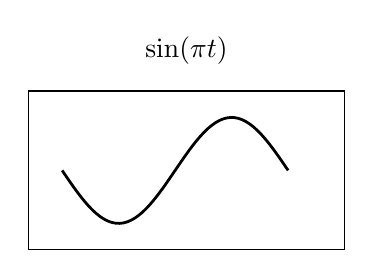
\begin{tikzpicture}
    \begin{axis}[width=5.6cm, height=3.6cm, xmin=-1.3, xmax=1.5, ymin=-1.5, ymax=1.5,
        xtick=\empty, ytick=\empty, title={$\sin(\pi t)$}]
      \addplot[black, line width=1pt, domain=-1:1, samples=60] {sin(180*x)};
    \end{axis}
  \end{tikzpicture}
\end{minipage}

\begin{center}
  \begin{tikzpicture}
    \begin{axis}[width=11cm, height=4.4cm, xmin=-4.6, xmax=4.9, ymin=-0.45, ymax=1.4,
        xtick={-3,-2,-1,1,2,3,4}, ytick={1}, xlabel={$t$}, ylabel={$\mathrm{sinc}(t)$}]
      \addplot[black, line width=1pt, domain=-4.5:4.5, samples=180] {sin(180*x)/(pi*x)};
      \addplot[only marks, mark=*, kirmizikalem, mark size=1.4pt] coordinates {(0,1)};
    \end{axis}
  \end{tikzpicture}
\end{center}

\begin{align*}
\textcolor{kirmizikalem}{\ast}\ \ (t=k)\in\mathbb{Z}-\{0\} &\Rightarrow \mathrm{sinc}(k)=\frac{\sin(k\pi)}{k\pi}=0 \\
t=0 &\Rightarrow \mathrm{sinc}(0)=\frac{\sin(0)}{0}=\frac{0}{0} \\
&\qquad\text{Hopital: } \lim_{t\to 0}\frac{\pi\cos(\pi t)}{\pi}=1
\end{align*}
\[ \mathrm{sinc}(-t)=\mathrm{sinc}(t) \]

\sayfa{7}
\subsection{İşaret fonksiyonu}
(Sign / Signum function)\footnote{Claude notu: Aşağıdaki $\mathrm{Sgn}(t)$ tanımında üçüncü satır ($0$, $t=0$) orijinalde kırmızı kalemle çizilerek iptal edilmiş.}
\[ \mathrm{Sgn}(t)=\begin{cases} 1 & t>0 \\ -1 & t<0 \\ \textcolor{kursunkalem}{0} & \textcolor{kursunkalem}{t=0}\end{cases} \]
\begin{center}
  \begin{tikzpicture}
    \begin{axis}[width=7.6cm, height=4.4cm, xmin=-2.3, xmax=2.6, ymin=-1.6, ymax=1.7,
        xtick=\empty, ytick={-1,1}, xlabel={$t$}, ylabel={$\mathrm{Sgn}(t)$}]
      \addplot[murekkep, line width=1.2pt] coordinates {(-2.3,-1) (0,-1)};
      \addplot[murekkep, line width=1.2pt] coordinates {(0,1) (2.4,1)};
    \end{axis}
  \end{tikzpicture}
\end{center}
\begin{align*}
\mathrm{Sgn}(t) &= u(t)-u(-t) \\
\textcolor{kirmizikalem}{\ast}\ \ u(t) &= \tfrac{1}{2}\bigl(1+\mathrm{Sgn}(t)\bigr)
\end{align*}

\subsection{Dürtü işareti}
(Impulse (Delta) Signal)

\noindent
\begin{minipage}[c]{0.5\linewidth}
  \centering
  \begin{tikzpicture}
    \begin{axis}[width=5.6cm, height=3.4cm, xmin=-1.8, xmax=2, ymin=-0.4, ymax=1.5,
        xtick=\empty, ytick=\empty, xlabel={$t$}, ylabel={$\delta(t)$}]
      \draw[-{Stealth[length=2.4mm]}, line width=1.4pt] (axis cs:0,0) -- (axis cs:0,1);
    \end{axis}
  \end{tikzpicture}
\end{minipage}\hfill
\begin{minipage}[c]{0.46\linewidth}
  \[ \delta(t)=\begin{cases} \infty, & t=0 \\ 0, & t\neq 0\end{cases} \]
\end{minipage}

Alan $=$ Şiddet $=\displaystyle\int_{-\infty}^{+\infty}\delta(t)\,dt=1$\footnote{Claude notu: Orijinalde kutudaki integralden bu satırın sonundaki ``$=1$'' ifadesine pembe bir ok çizilmiş; okun üzerindeki küçük not güçlükle okundu (muhtemelen ``1 ise'').}

\formulkutu[$f(t)$ $t=0$'da sürekliyse]{\underset{\text{(sifting property)}}{\int_{-\infty}^{+\infty}f(t)\,\delta(t)\,dt=f(0)}}

\sayfa{8}
\textcolor{kirmizikalem}{sinc de bu koşulu sağlıyor}
\[ \textcolor{kirmizikalem}{\ast}\ \delta(t)=\lim_{\varepsilon\to 0}\frac{1}{\varepsilon}\,\Pi\!\left(\frac{t}{\varepsilon}\right) \]
\begin{center}
  \begin{tikzpicture}
    \begin{axis}[width=12cm, height=5.6cm, xmin=-0.75, xmax=1.35, ymin=-0.6, ymax=4.8,
        xtick={-0.5,-0.25,0.25,0.5}, xticklabels={$-1/2$,$-1/4$,$1/4$,$1/2$}, ytick={1}, xlabel={$t$}]
      \addplot[black, line width=1pt] coordinates {(-0.5,0) (-0.5,1) (0.5,1) (0.5,0)};
      \addplot[kirmizikalem, line width=1pt] coordinates {(-0.25,0) (-0.25,2) (0.25,2) (0.25,0)};
      \addplot[kirmizikalem!55, line width=1pt] coordinates {(-0.125,0) (-0.125,4) (0.125,4) (0.125,0)};
      \node[kirmizikalem!55, anchor=north, font=\scriptsize] at (axis cs:-0.125,-0.5) {$-1/8$};
      \node[kirmizikalem!55, anchor=north, font=\scriptsize] at (axis cs:0.125,-0.5) {$1/8$};
      \node[anchor=west] at (axis cs:0.62,1) {$\Pi(t)$};
      \node[kirmizikalem, anchor=west] at (axis cs:0.34,2.1) {$2\Pi(2t)$};
      \node[kirmizikalem, anchor=west] at (axis cs:0.95,2.5) {$\varepsilon=\frac{1}{2}$};
      \node[kirmizikalem!55, anchor=west] at (axis cs:0.25,4.1) {$4\Pi(4t)$};
    \end{axis}
  \end{tikzpicture}
\end{center}

\noindent\textbf{Özellikleri:} sifting/sampling property
\[ \textcolor{kirmizikalem}{\ast}\ \ \text{1)}\quad f(t)\,\delta(t-t_0)=f(t_0)\,\delta(t-t_0),\qquad t_0=\text{sabit} \]

\elcizimi[0.9]{sekiller/Ders2-s8-1.png}[8]

\textcolor{kirmizikalem}{$\ast$} 2) $f(t)$ $t=t_0$'da sürekli olmak üzere
\[ \int_a^b f(t)\,\delta(t-t_0)\,dt=\begin{cases} f(t_0) & a<t_0<b \\ 0 & \text{diğer}\end{cases} \]
\[ f(t)=1\ \longrightarrow\ \int_a^b\delta(t-t_0)\,dt=\begin{cases} 1 & \text{$0<t_0<b$\footnotemark} \\ 0 & \text{diğer}\end{cases} \]
\footnotetext{Claude notu: muhtemelen $a<t_0<b$ olmalı.}
\begin{center}
  \begin{tikzpicture}
    \begin{axis}[width=6.4cm, height=3cm, xmin=-1, xmax=3.4, ymin=-0.3, ymax=1.7,
        xtick={-0.6,1.2,2.6}, xticklabels={$a$,$t_0$,$b$}, ytick=\empty]
      \draw[-{Stealth[length=2.2mm]}, line width=1.2pt] (axis cs:1.2,0) -- (axis cs:1.2,1.1)
        node[above right] {$\delta(t-t_0)$};
    \end{axis}
  \end{tikzpicture}
\end{center}
\[ f(t_0)\,\delta(t-t_0) \]
\[ f(t_0)\underbrace{\int_a^b\delta(t-t_0)\,dt}_{1,\ a<t_0<b} \]

\sayfa{9}
\[ \text{3)}\ \ \forall a\neq 0 \qquad \delta(at)=\frac{1}{|a|}\,\delta(t) \]
\begin{align*}
a=-1 &\Rightarrow \delta(-t)=\frac{1}{|-1|}\,\delta(t) \\
&\Rightarrow \delta(-t)=\delta(t) \quad \text{çift fonksiyondur.}
\end{align*}
\[ \text{4)}\ \ f(t)\circledast\delta(t)=f(t) \]
\[ \textcolor{kirmizikalem}{\ast}\ f(t)\circledast\delta(t-t_0)=f(t-t_0) \]
\[ x(t)\circledast y(t)=\int_{-\infty}^{\infty}x(\tau)\,y(t-\tau)\,d\tau \]
\begin{align*}
f(t)\circledast\delta(t) &= \int_{-\infty}^{+\infty}f(\tau)\,\delta(t-\tau)\,d\tau \\
&= \int_{-\infty}^{+\infty}f(\tau)\,\delta(\tau-t)\,d\tau \\
&= f(t)
\end{align*}
\begin{align*}
f(t)\circledast\delta(t-t_0) &= \int_{-\infty}^{+\infty}f(\tau)\underbrace{\delta(t-\tau-t_0)}_{\delta\left(\tau-\underbrace{(t-t_0)}_{\text{sabit}}\right)}d\tau \\
&= f(t-t_0)
\end{align*}
\[ \text{5)}\ \ \int_{-\infty}^{t}\delta(\tau)\,d\tau=\begin{cases} 1, & t>0 \\ 0, & t<0\end{cases} \ \equiv\ u(t) \]
\[ \int_{-\infty}^{t}\delta(\tau)\,d\tau=u(t)\ \xRightarrow{\ \frac{d}{dt}\ }\ \frac{d}{dt}\,u(t)=\delta(t) \]

\sayfa{10}
\subsection{Ortogonal (Dik) / Ortonormal işaretleri}
Eğer $\psi_1(t),\ \psi_2(t),\ \ldots\ \psi_n(t)$ işaretleri $[t_1,t_2]$ aralığında
\[ \int_{t_1}^{t_2}\psi_m(t)\,\psi_n^{*}(t)\,dt=\begin{cases} 0 & m\neq n \\ E_m & m=n\end{cases} \]
sağlıyorsa ortagonaldır ilaveten $\forall m\ E_m=1$ ise işaretler ortonormaldır

\begin{ornek}
  \noindent
  \begin{minipage}[c]{0.48\linewidth}
    \centering
    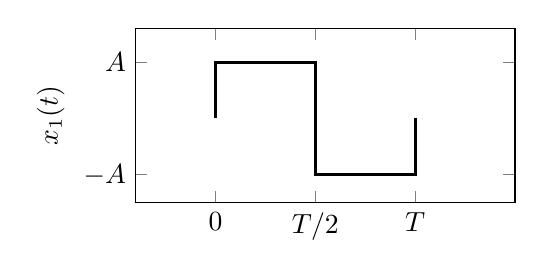
\begin{tikzpicture}
      \begin{axis}[width=6.4cm, height=3.8cm, xmin=-0.8, xmax=3, ymin=-1.5, ymax=1.6,
          xtick={0,1,2}, xticklabels={$0$,$T/2$,$T$}, ytick={-1,1}, yticklabels={$-A$,$A$}, ylabel={$x_1(t)$}]
        \addplot[black, line width=1.1pt] coordinates {(0,0) (0,1) (1,1) (1,-1) (2,-1) (2,0)};
      \end{axis}
    \end{tikzpicture}
  \end{minipage}\hfill
  \begin{minipage}[c]{0.48\linewidth}
    \centering
    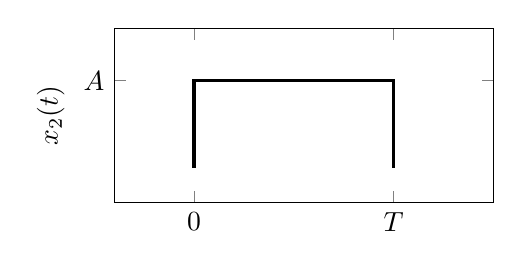
\begin{tikzpicture}
      \begin{axis}[width=6.4cm, height=3.8cm, xmin=-0.8, xmax=3, ymin=-0.4, ymax=1.6,
          xtick={0,2}, xticklabels={$0$,$T$}, ytick={1}, yticklabels={$A$}, ylabel={$x_2(t)$}]
        \addplot[black, line width=1.1pt] coordinates {(0,0) (0,1) (2,1) (2,0)};
      \end{axis}
    \end{tikzpicture}
  \end{minipage}
  \begin{align*}
    \int_0^T x_1(t)\cdot x_2(t)\,dt &= \underbrace{\int_0^{T/2}A^2\,dt}_{A^2\,\frac{T}{2}} + \underbrace{\int_{T/2}^{T}A(-A)\,dt}_{-A^2\left(T-\frac{T}{2}\right)} \\
    &= 0 \quad\Rightarrow\ \text{Ortagonel}
  \end{align*}
  \begin{align*}
    E_1 &= \int_0^T x_1^2(t)\,dt \\
    &= \int_0^T A^2\,dt = A^2T = E_2
  \end{align*}
\end{ornek}

\sayfa{11}
Ortonormal olması için iki işaretin genlikleri $\sqrt{A^2T}$ ye bölmemiz lazım. Böylece enerjileri 1 olur.
\begin{align*}
x(t) &\to E_x \\
x_N(t)=\frac{x(t)}{\sqrt{E_x}} &\to E_{x_N}=\int_{-\infty}^{\infty}x_N^2(t)\,dt \\
&\hspace{1.1cm}=\frac{1}{E_x}\underbrace{\int_{-\infty}^{\infty}x(t)^2\,dt}_{E_x} \\
&\hspace{1.1cm}=1
\end{align*}

\subsection{Sistemler}
Sistem, bir düzenektir.
\[ y(t)=T\bigl[x(t)\bigr] \]
\begin{center}
  \begin{tikzpicture}[line width=0.9pt]
    \node[draw, minimum width=2.4cm, minimum height=1.5cm] (T) at (0,0) {$T[\ \ ]$};
    \draw[-{Stealth[length=2.2mm]}] (-3.4,0) -- (T.west) node[midway, below] {$x(t)$};
    \draw[-{Stealth[length=2.2mm]}] (T.east) -- ++(2.4,0) node[right] {$y(t)$};
  \end{tikzpicture}
\end{center}

\noindent
\begin{tabular}{@{}p{0.47\linewidth}p{0.47\linewidth}@{}}
  \textcolor{kirmizikalem}{$\ast$} Sürekli zamanlı s. & $\times$ Ayrık zamanlı s. \\[1mm]
  \quad $y(t)=\dfrac{d}{dt}\,x(t)$ & \quad $y[n]=x[n]-x[n-1]$ \\[5mm]
  \textcolor{kirmizikalem}{$\ast$}- Lineer & $\times$ Lineer olmayan
\end{tabular}

$\alpha,\beta$ skaler
\begin{align*}
y_1(t) &= T[x_1(t)] \\
y_2(t) &= T[x_2(t)]
\end{align*}
\begin{align*}
x_3(t) &= \alpha x_1(t)+\beta x_2(t) \\
\to\ y_3(t) &= T[x_3(t)] \\
&= T[\alpha x_1(t)+\beta x_2(t)] \\
&= \alpha T[x_1(t)]+\beta T[x_2(t)] \\
&= \alpha y_1(t)+\beta y_2(t)
\end{align*}

\sayfa{12}
Eğer bir sistemin $x_1(t)$ ve $x_2(t)$ ye cevabını biliyorsanız sonsuz tane $x_3(t)$ $x_1$ ve $x_2$'nin linear kombinasyonu cinsinden yazılabilir.

\medskip
\noindent $y(t)=\dfrac{d}{dt}\,x(t)$ \ \underline{lineer} \\[1mm]
$y(t)=x^2(t)$ \ \underline{lineer değil}

\medskip
\noindent
\begin{tabular}{@{}p{0.47\linewidth}p{0.47\linewidth}@{}}
  \textcolor{kirmizikalem}{$\ast$} Zamanla Değişen S. & $\times$ Zamanla Değişmeyen S. \\
  \quad (Time varient) & \quad (Time Inveriant)
\end{tabular}

\[ \forall t,\ x(t)\qquad\begin{aligned}[t] y(t)&=T[x(t)] \\ T[x(t-t_0)]&=y(t-t_0) \\ &\Rightarrow\ \text{Zamanla Değişmen (TI)}\end{aligned} \]

\begin{ornek}
  $y(t)=t\,x(t)$
  \begin{align*}
    x_1(t) &\to y_1(t)=t\,x_1(t) \\
    x_2(t)=x(t-t_0) &\to y_2(t)=t\,x_2(t)=t\,x_1(t-t_0) \\
    &\hphantom{\to\ }y_1(t-t_0)\overset{\neq}{=}(t-t_0)\,x_1(t-t_0)
  \end{align*}
  $\Rightarrow$ Zamanla Değişen bir işaret
\end{ornek}

\noindent\textbf{Ödev}\quad $y(t)=x(t+1)$ \qquad\qquad Zamanla değişmeyen sistem
\begin{align*}
x_1(t) &\to y_1(t)=x_1(t+1) \\
x_2(t)=x_1(t+1-t_0) &\to y_2(t)=x_2(t)=x_1(t+1-t_0)\footnotemark \\
&\hphantom{\to\ }y_1(t-t_0)\overset{\prime\prime}{=}x_1(t+1-t_0)
\end{align*}
\footnotetext{Claude notu: muhtemelen $x_2(t)=x_1(t-t_0)$ ve $y_2(t)=x_2(t+1)=x_1(t+1-t_0)$ olmalı.}
Zamanla değişmeyen sistem

\medskip
\noindent\textcolor{kirmizikalem}{$\ast$} Lineer + Zamanla değişmen S $=$ LZD sistem \\
(Lineer Time Inavariant (LTI) )

\sayfa{13}
\subsection{Nedensel (Casual) Sistem}
\[ y(t_0)=T\bigl[x(t),\ t\le t_0\bigr]\ \Rightarrow\ \text{Nedensel sistem} \]
Çıkışı sadece şimdiki ve geçmişteki ana bağlı çıkış olan sistemdir. Çıkış geleceğe bağlı değildir.

\begin{ornek}
  \begin{center}
    \begin{tikzpicture}[line width=0.9pt]
      \node[draw, minimum width=2.6cm, minimum height=1.5cm, align=center] (G) at (0,0) {Gecikme\\ $D$};
      \draw[-{Stealth[length=2.2mm]}] (-3.4,0) -- (G.west);
      \node at (-2.4,0.35) {$x(t)$};
      \draw[-{Stealth[length=2.2mm]}] (G.east) -- ++(1.8,0) node[right] {$y(t)=x(t-D)$};
    \end{tikzpicture}
  \end{center}
  $D\ge 0$ için nedensel
\end{ornek}

\subsection{Dürtü Cevabı (Impulse Response)}
\[ \text{LZD sistem}\ \Rightarrow\ y(t)=T\bigl[\delta(t)\bigr]=\underbrace{h(t)}_{\substack{\text{sistemin}\\\text{dürtü}\\\text{cevabı}}} \]
\begin{center}
  \begin{tikzpicture}[line width=0.9pt]
    \node[draw, minimum width=1.6cm, minimum height=1.4cm] (H) at (0,0) {$h(t)$};
    \draw[-{Stealth[length=2.2mm]}] (-3.4,0) -- (H.west) node[midway, below] {$x(t)$};
    \draw[-{Stealth[length=2.2mm]}] (H.east) -- ++(3.2,0);
  \end{tikzpicture}
\end{center}
\begin{align*}
y(t) &= x(t)\circledast h(t) \\
&= \int_{-\infty}^{\infty}x(\tau)\,h(t-\tau)\,d\tau \\
&= \int_{-\infty}^{\infty}x(t-\tau)\,h(\tau)\,d\tau
\end{align*}
LZD sistemin nedensel olması için gerek ve yeter şart $h(t)=0,\ t<0$

\textcolor{kirmizikalem}{ispatı nedir??}

\end{document}
